\documentclass[10pt]{article}

\usepackage[T1]{fontenc}
\usepackage[utf8]{inputenc}
\usepackage[french]{babel} 
\usepackage{graphicx} % images
\usepackage{hyperref} % liens
\usepackage{amsmath} % pour le texte dans les formules
\usepackage[squaren,Gray]{SIunits} % pour afficher les nombres sans le mode math qui est moche
\usepackage{float}
\usepackage{hyperref}
\usepackage{fullpage}
\usepackage[final]{pdfpages} % Package afin d'inculre des pdf dans le rapport

\frenchspacing

\title{Projet 3 - Gestionnaire de code-barres CB2D}
\date{3 décembre 2014}
\author{Robin Gielen, Julien Banken et Jérémy Gossiaux}

\newcommand{\HRule}{\rule{\linewidth}{0.5mm}}


\begin{document}

\begin{titlepage}
\begin{center}

% Upper part of the page. The '~' is needed because \\
% only works if a paragraph has started.

\textsc{\Large LSINF 1102 - Résolution informatiques de problèmes}\\[0.5cm]

% Title
\HRule \\[0.4cm]
{ \huge \bfseries Projet 3 - Gestionnaire de code-barres CB2D \\[0.4cm] }

\HRule \\[1.5cm]

{\large \today}

\vfill


\begin{figure}[!h]
	\centering
	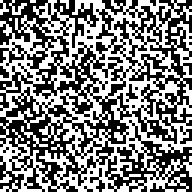
\includegraphics[width=0.4\textwidth]{images/barcode.png}
	\caption{Code-barre}  
	\label{Code-barre}
\end{figure}


% Author and supervisor
\noindent
\begin{minipage}{0.4\textwidth}
\begin{flushleft} \large 
\emph{Auteurs:}\\
Robin Gielen, Julien Banken, Jérémy Gossiaux \textsc{} 
\end{flushleft}
\end{minipage}%
\begin{minipage}{0.4\textwidth}
\begin{flushright} \large
\emph{Tuteur:} \\
Xavier \textsc{Carpent}
\end{flushright}
\end{minipage}



\end{center}
\end{titlepage}

\tableofcontents

\newpage

\section{Abstract}

%Francais 
%
%Dans le cadre de notre première année en bachelier en sciences informatiques, nous avons eu à réaliser un projet de groupe. Ceci impliquant une quantité de travail non négligeable, une cohésion de groupe nécessaire pour avancer efficacement et l'apprentissage de nouvelles notions. L'objectif du projet était de créer un programme capable de lire et de générer des code-barres à deux dimensions appelés CB2D. Les différentes tâches étaient la création du programme en lui même, une interrogation sur les conséquences d'un passage aux code-barres QR-code et finalement la rédaction de ce rapport. A terme, nous sommes parvenus à fournir un programme qui respecte effectivement les spécifications du cahier des charges établis au début du projet. 

%Anglais 

In the context of our first bachelor year in ???computer science???, we had to carry out a group project. This project involving a significant amount of work, a group cohesion needed to work properly and efficiently together and the learning of new concepts related to ???computer science???.The main objective was to create a programme capable of reading and generating 2D bare-codes with a specific format named CB2D. The different tasks were to design and code the programme, to think about the consequences of using QR-Codes instead of CB2D in our programme and finally the writing of this report about our work. In the end, we successfully created the demanded programme according to the specifications. ???As for??? the implementation of QR-Code, we discuss about it in our report.



\section{Introduction}

Dans le cadre du cours de résolution informatique de problèmes, la société N-Side a demandé aux étudiant de développer un programme capable de lire et de générer des code-barres au format spécifique CB2D. Le rapport suivant à pour but d'expliquer dans le détail les spécifications du programme ainsi que la manière de l'utiliser. Tout d'abord, le rapport détaillera le cahier des charges, avec ses fonctions principales et ses contraintes. Ensuite, le rapport montrera la façon dont l'utilisateur pourra intéragir avec le programme et les différentes options qui se présenteront à lui. Par après, le rapport expliquera les différentes fonctionnalités du code, les choix qui ont été fait et les justifications de ces choix. Enfin, le rapport analysera les conséquences d'un passage du format CB2D au format QR-Code pour le programme et une section expliquera les détails du planning. 


\newpage 

\section{Cahier des charges}

Lors de la rédaction de notre cahier des charges, nous avons décidé de le présenter sous la forme suivante : \\
Tout d'abord une partie reprenant les fonctions principales en général, ensuite une partie précisant les différentes spécifications propres à chacunes de nos fonctions principales et enfin une partie contenant les contraintes spécifiques à notre programme. 

\subsection{Fonctions Principales}

\begin{itemize}
\item Générer des code-barres CB2D à partir d'un texte
\item Lire des code-barres CB2D et en extraire les informations
\item Intégrer une fonction de vérification et de correction des code-barres CB2D
\end{itemize}

\subsection{Niveaux de Fonctions Principales}

\subsubsection{Générer des code-barres CB2D} 

La première chose que le programme doit effectuer lors de la génération d'un CB2D est d'analyser l'information à stocker afin d'en extraire plusieurs informations : \\

\begin{itemize}
\item La taille de l'information à stocker
\end{itemize}
Nous cherchons à minimiser la taille du CB2D pour ne pas perdre de l'espace inutilement. \\

\begin{itemize}
\item Le type de données à stocker
\end{itemize}
Il existe en effet plusieurs type de données pris en compte : 

	\begin{enumerate}
	\item Texte ASCII 7-bits (Norme ISO 646)
	\item Texte ASCII étendu (Norme ISO 8859-1)
	\item URL (Norme RFC 3986)
	\end{enumerate}

\begin{itemize}
\item Le type de compression appliqué aux données contenues
\end{itemize}

Nous n'avons actuellement pas de compression appliquée à nos données, mais il est tout a fait possible d'ajouter cette fonction au programme dans le futur. \\

Mais le programme doit également mettre en place le système de correction, que nous présentons dans la section "3.2.3 Intégrer une fonction de correction des CB2D", qui sera utilisé lors d'une futur lecture du CB2D.

\subsubsection{Lire des code-barres CB2D}

Lors de la lecture des CB2D, le programme doit effectuer une vérification grâce à l'algorithme de correction. En effet, le programme doit s'assurer un minimum que le CB2D qu'il s'apprete à lire n'est pas endommager.
De plus, le programme doit être capable d'identifier le type de compression et le type de données stockées dans le CB2D afin de pouvoir lire ce dernier à pleine efficacité. Les différentes informations relatives à ces données ayant déjà été citées plus haut dans la section "3.2.1 Générer des code-barres CB2D".

\subsubsection{Intégrer une fonction de correction des CB2D}

Le programme inclut, en effet, un algorithme de correction qui va permettre de savoir si le CB2D a été altéré entre le moment où il a été généré et le moment où il va être lu. 
Cet algorithme fonctionne de la manière suivante : \\
Lors de l'écriture du CB2D, le programme garde à sa disposition la première ligne et la première colonne pour le correcteur. Lorsque le CB2D est pret à être imprimé, le programme va regarder la parité de chaque ligne et de chaque colonne et indiqué celle-ci dans la première ligne/colonne correspondante. Ainsi, lors de la lecture du CB2D, le programme pourra vérifier si la parité est respectée. Trois cas peuvent alors se présenter : 
\begin{itemize}
\item Il n'y a pas d'erreur \textbf{détectée} par le programme
\item Une seul erreur est \textbf{détectée} par le programme
\item Plusieurs erreurs sont \textbf{détectées} par le programme
\end{itemize} 
Cet algorithme est surtout efficace pour détecter les erreurs, et non pas pour corriger totalement un CB2D. En effet, il est tout à fait possible que le programme ne détecte qu'une seule erreur (alors que plusieurs sont présentes) si plus d'une section du CB2D a été déteriorée. Ou encore de ne pas détecter d'erreur malgré qu'une soit bien présente. 
Dans le cas ou le programme détecte une seule erreur, il pourra la réparer, mais si le programme détecte plusieurs erreurs, il ne pourra qu'afficher les numéros des lignes et colonnes concernées sans pouvoir le corriger avec certitude. \\
Cependant, cet algorithme a pour avantage de détecter avec une précision appréciable si le CB2D a été altéré ou pas, et donc permettre d'extraire les informations tout en informant l'utilisateur d'une possible corruption de celles-ci.

\subsection{Contraintes}

Les contraintes sont les suivantes : 

\begin{itemize}
\item La taille d'un code-barre sera de :
	\begin{enumerate}
	\item 32 * 32 
	\item 64 * 64 
	\item 128 * 128 
	\item 256 * 256
	\end{enumerate}
\item La lecture et la génération devra être effectuée en moins de 2 secondes
\item Le CB2D devra être chargé à partir d'une image
\item Le texte qui sera imprimé ne devra pas depasser 8182 caractères
\end{itemize}



\newpage
\section{Installation et utilisation}

Le programme, qui est programmé en Java, est assez simple d'utilisation. En effet, ce dernier ne requiert aucune installation particulière, mais plutot une mise en place de certains éléments. 

\subsection{Installation}

\subsection{Utilisation}

Lors du lancement du programme, l'utilisateur se verra demandé ce qu'il souhaite faire : 
\begin{itemize}
\item Lire un code-barre à partir d'un fichier image
\item Générer un code-barre à partir d'un texte qu'il devra fournir
\end{itemize}

Via la commande, l'utilisateur choisira donc l'action qu'il souhaite effectuer (cfr figure 1). Ensuite, l'utilisateur sera guidé à travers les différentes étapes pour la lecture et la génération de CB2D. L'utilisateur n'aura aucun problème pour utiliser le programme car l'interface de ce dernier est facile à comprendre et très intuitive. 

\begin{figure}[!h]
	\centering
	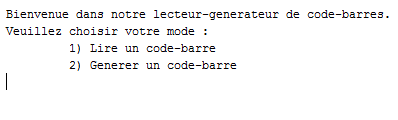
\includegraphics[width=0.7\textwidth]{images/choixMode.png}
	\caption{Choix du mode d'utilisation}  
	\label{Choix du mode d'utilisation}
\end{figure}



\subsection{Lecture}

Si l'utilisateur choisit de lire un code-barre, il lui sera demandé de spécifié le chemin d'accès au fichier image qui contient le CB2D. Ensuite, l'utilisateur n'aura plus qu'à attendre que le programme décode le CB2D et qu'il en extraie les informations contenues.

Ensuite, les informations seront présentées à l'utilisateur.

\subsection{Génération}

Si en revanche l'utilisateur choisit de générer un code-barre, il devra alors fournir les informations à stocker, sous forme de texte, au programme. Le programme va ensuite encoder les informations et les transformer en CB2D, qui sera ensuite imprimé et sauvegardé dans un fichier image.
\input{5FonctionnalitéDuCode.tex}
\newpage

\section{Migration vers les codes QR}

Il existe plusieurs avantages et désavantages pour l'utilisation des codes-QR, voici une liste non exhaustive des points les plus importants que nous avons relevés.

\subsection{Avantages}

\begin{itemize}
\item Il existe déjà de nombreuses applications capables de lire les QR Codes sur de nombreuses plateformes
\end{itemize}
Cela évite de devoir développer une application par nous même pour chaque plateforme.

\begin{itemize}
\item Permet d'effectuer un virement direct via son téléphone portable
\end{itemize}
Cela permetrait éventuellement de payer directement les médicaments dans les pharmacies ou les hopitaux grâce à un simple scan du QR code.

\begin{itemize}
\item Les codes QR peuvent généralement être lus même si 25$\%$ de la surface du QR code est effacée
\end{itemize}
Ce pourcentage de surface pouvant être abimé est excellent. Cela permet d'assurer une lecture des codes QR avec une grande efficacité.


\subsection{Désavantages}

\begin{itemize}
\item La quantité d'information que l'on peut stockée est limitée à environ 500 mots
\end{itemize}
Cette quantité est moins importante que lors du stockage d'informations dans un CB2D. Hors le stockage d'information est le but premier de l'utilisation des CB2D.
\newpage

\section{Planning}

\begin{figure}[!h]
	\centering
	\includegraphics[width=0.85\textwidth]{images/planning.pdf} 
	\label{Planning}
\end{figure}


\section{Conclusion}

Conclusion


\newpage

\section{Annexe}


\subsection{Cahier des Charges}

%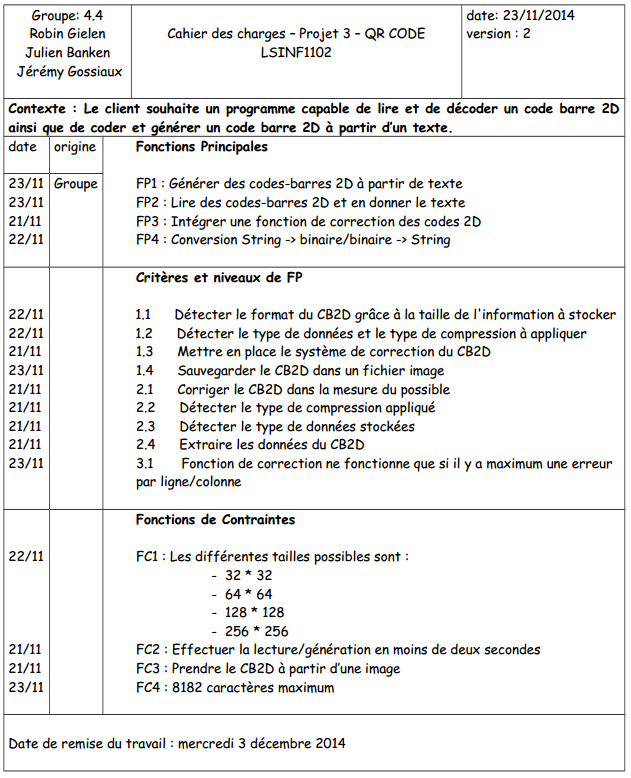
\includepdf{images/CahierDesCharges.pdf}

\begin{figure}[!h]
	\centering
	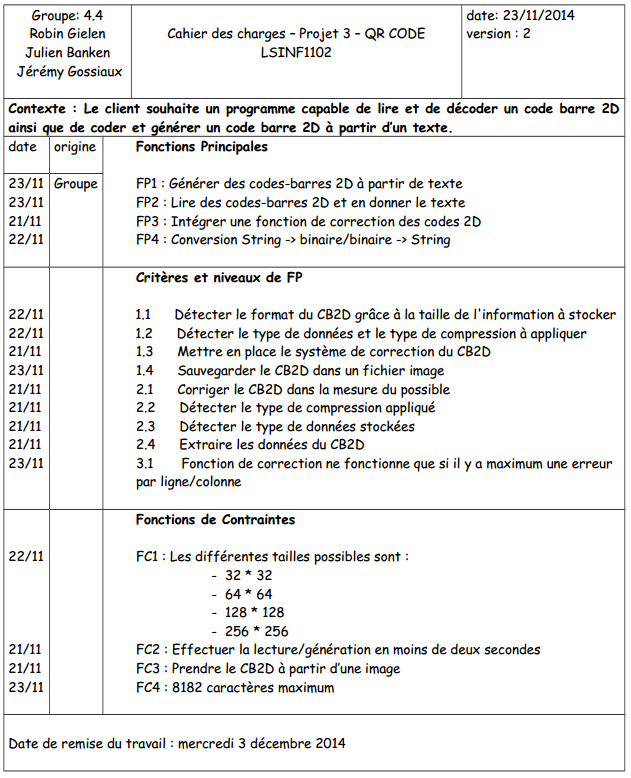
\includegraphics[width=0.85\textwidth]{images/CahierDesCharges.pdf}
	\label{Cahier des charges}
\end{figure}


\end{document}
